
\chapter{Stochastic Processes}

In the previous chapter Brownian motion appeared twice, and in two rather different guises: as a macroscopic diffusion process, governed by a partial differential equation for a density, and as the microscopic, erratic trajectory of a suspended particle.
It is natural to ask what these two descriptions have in common, and whether they are instances of something more general.
They are.
In this chapter we step back and develop the general formalism of \emph{stochastic processes}, of which Brownian motion is the most fundamental example.
Our goal is to construct, in full generality, the equation that governs the evolution in time of the probability density of a random variable, and to identify the conditions under which this equation takes the manageable form of a \emph{Fokker--Planck equation}.
Everything we do later in this book --- from option pricing to the distribution of wealth --- rests on the machinery built here.


\section{General formalism}

A \emph{stochastic process} is a system that evolves in time in a probabilistic way.
Physically, it is the probabilistic counterpart of a dynamical system: the time evolution is still governed by a law, but the law prescribes probabilities rather than certainties.
% CLAUDE NOTE: the "physical definition" sentence follows the course slides
% (Processi Stocastici: definizioni & classificazione), added 2026-07-06.
Formally, it is a family of random variables
\begin{equation}
\{X(t),\, t\in T\},
\end{equation}
indexed by a time parameter $t$ that runs over a (non-numerable) set $T$.
Two cases occur in practice.
If time is \emph{discrete}, $T=\mathbb{N}$, the process is a sequence $X(t=t_n)=X_n$; if time is \emph{continuous}, $T=\mathbb{R}^+$, the process is a function $X(t)=x(t)$.
We will mostly work in continuous time, although discretization will reappear whenever we need to actually compute something.

A particular sequence of values produced by the process is a \emph{realization}, or \emph{trajectory}.
When the sequence comes from real observations, one speaks of a \emph{historical time series}.
The set of all possible realizations is called the \emph{ensemble} (or \emph{phase space}), visualized in Figure~\ref{fig:ensemble}: a stochastic process is an infinite family of functions evolving randomly in time, and cutting the family at a fixed time $t_0$ defines the random variable $X(t_0)$.
The distinction matters: an experimentalist --- or a trader --- only ever observes \emph{one} realization, whereas the theory speaks about the whole ensemble.
We will meet the consequences of this tension more than once.

% Figure after the course slides (Processi Stocastici: definizioni & classificazione);
% generated by images/code_for_images/ensemble.py
\begin{figure}[h!]
\centering
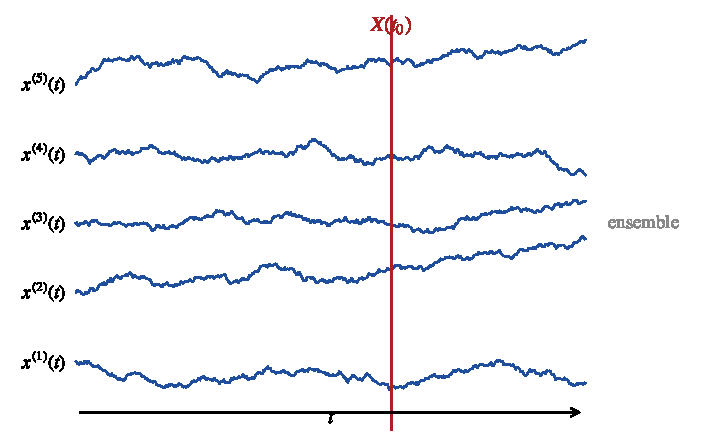
\includegraphics[width=0.7\textwidth]{images/ensemble.pdf}
\caption{Realizations and ensemble. Each curve $x^{(k)}(t)$ is one realization of the same stochastic process; the collection of all of them is the ensemble (phase space). Fixing a time $t_0$ (vertical cut) turns the process into an ordinary random variable $X(t_0)$, whose statistics is taken \emph{across} the realizations. Generated by \texttt{images/code\_for\_images/ensemble.py}.}
\label{fig:ensemble}
\end{figure}

At the statistical level, the process is completely characterized by its \emph{joint probability density}
\begin{equation}
P_n(x_n,t_n;\,x_{n-1},t_{n-1};\dots;x_1,t_1) \equiv P_n,
\end{equation}
which gives the probability density of observing the value $x_1$ at time $t_1$, the value $x_2$ at time $t_2$, and so on.
We adopt throughout the \emph{forward} ordering of the times; the backward ordering gives an equivalent description.
That the whole hierarchy $\{P_n\}$ really is all there is to know is the content of a classical result.

\medskip
\noindent\textbf{Theorem (Kolmogorov).}\cite{Kolmogorov1931}
\emph{A stochastic process is uniquely defined once the finite-dimensional joint probability density is assigned for every finite set of times $\{t_1,t_2,\dots,t_n\}\in T$.}
\medskip

The hierarchy of joint densities cannot be arbitrary, however: it must satisfy four consistency conditions.
\begin{enumerate}
    \item \textbf{Positivity}: each density is non-negative,
    \begin{equation}
    P_n \ge 0.
    \end{equation}
    \item \textbf{Symmetry}: the density is invariant under any permutation of its $(x_i,t_i)$ pairs,
    \begin{equation}
    P_n(\dots;x_i,t_i;\dots;x_j,t_j;\dots) = P_n(\dots;x_j,t_j;\dots;x_i,t_i;\dots).
    \end{equation}
    \item \textbf{Completeness} (marginalization): integrating out the most recent variable lowers the order of the hierarchy,
    \begin{equation}
    \int_{-\infty}^{\infty} P_n(x_n,t_n;\dots;x_1,t_1)\,dx_n = P_{n-1}(x_{n-1},t_{n-1};\dots;x_1,t_1).
    \end{equation}
    \item \textbf{Normalization}: the one-time density integrates to one,
    \begin{equation}
    \int_{-\infty}^{\infty} P_1(x,t)\,dx = 1.
    \end{equation}
\end{enumerate}
These conditions look innocuous, but completeness in particular will do real work for us shortly: it is the seed of the Chapman--Kolmogorov equation.

Two special classes of processes deserve a name.
A process is \emph{stationary} when the joint density is invariant under a global translation of all the times,
\begin{equation}
P_n(x_n,t_n+\Delta t;\dots;x_1,t_1+\Delta t) = P_n(x_n,t_n;\dots;x_1,t_1),
\end{equation}
so that only time \emph{differences} matter; in particular the one-time density becomes time independent, $P(x,t)=P(x)$.
A process is instead \emph{purely random} when there is no correlation at all between different times: for every $m$ and every $t_1\le\dots\le t_m$,
\begin{equation}
P(x_m,t_m\mid x_{m-1},t_{m-1};\dots;x_1,t_1) = P(x_m,t_m),
\end{equation}
so that the joint density factorizes completely,
\begin{equation}
P_m(x_m,t_m;\dots;x_1,t_1) = \prod_{i=1}^{m} P(x_i,t_i).
\end{equation}
A purely random process has no dynamics worth the name: each instant is drawn afresh, oblivious of everything that came before.

In writing the last definitions we have used the \emph{conditional} density, defined as
\begin{equation}
P(x_m,t_m\mid x_{m-1},t_{m-1};\dots;x_1,t_1) := \frac{P_m(x_m,t_m;x_{m-1},t_{m-1};\dots;x_1,t_1)}{P_{m-1}(x_{m-1},t_{m-1};\dots;x_1,t_1)},
\end{equation}
from which the \emph{Bayes theorem} follows immediately,
\begin{equation}
P_2(x_2,t_2;x_1,t_1) = P(x_2,t_2\mid x_1,t_1)\,P_1(x_1,t_1).
\end{equation}
The conditional density answers the question that any observer actually asks: \emph{given} what I have seen so far, what happens next?


\section{Markov processes and the Chapman--Kolmogorov equation}

Between the two extremes of a purely random process (no memory at all) and a general process (arbitrarily long memory) lies the class that dominates applications.
A process is a \emph{Markov process} when the conditional density depends only on the most recent time,
\begin{equation}
P(x_m,t_m\mid x_{m-1},t_{m-1};\dots;x_1,t_1) = P(x_m,t_m\mid x_{m-1},t_{m-1}),
\qquad \forall m,\ \forall t_1\le\dots\le t_m.
\end{equation}
In words: knowledge of the present determines the statistics of the future, with no memory of the past.
A typical example is the tossing of coins in succession in time.
Whether \emph{prices} are Markovian is a far deeper question, and one to which we shall return in Chapter~5.

The Markov property has two consequences that between them carry the entire chapter.

\paragraph{1) Structure of the joint density.}
By definition of the conditional density,
\begin{equation}\begin{split}
P(x_m,t_m\mid x_{m-1},t_{m-1};\dots;x_1,t_1)
&= \frac{P_m(x_m,t_m;x_{m-1},t_{m-1};\dots;x_1,t_1)}{P_{m-1}(x_{m-1},t_{m-1};\dots;x_1,t_1)}\\
&= P(x_m,t_m\mid x_{m-1},t_{m-1}),
\end{split}\end{equation}
from which
\begin{equation}
P_m(x_m,t_m;\dots;x_1,t_1) = P(x_m,t_m\mid x_{m-1},t_{m-1})\,P_{m-1}(x_{m-1},t_{m-1};\dots;x_1,t_1).
\end{equation}
The same identity applied to $P_{m-1}$ gives
\begin{equation}
P_{m-1}(x_{m-1},t_{m-1};x_{m-2},t_{m-2};\dots) = P(x_{m-1},t_{m-1}\mid x_{m-2},t_{m-2})\,P_{m-2}(x_{m-2},t_{m-2};\dots),
\end{equation}
and therefore
\begin{equation}
P_m = P(x_m,t_m\mid x_{m-1},t_{m-1})\,P(x_{m-1},t_{m-1}\mid x_{m-2},t_{m-2})\,P_{m-2}.
\end{equation}
Iterating all the way down to $P_1$, we obtain
\begin{equation}
P_m(x_m,t_m;\dots;x_1,t_1) = \prod_{j=2}^{m} \underbrace{P(x_j,t_j\mid x_{j-1},t_{j-1})}_{\text{transition probability (in } t_j-t_{j-1})}\ \underbrace{P(x_1,t_1)}_{\text{assigned condition}}.
\end{equation}
This is a remarkable simplification.
A Markov process is entirely built out of two ingredients: the \emph{transition probabilities} $P(x_j,t_j\mid x_{j-1},t_{j-1})$, which propagate the process one step at a time, and the initial one-time density.
Instead of an infinite hierarchy of joint densities, we need to understand a single object --- the transition probability --- and everything else follows.

\paragraph{2) Linking points in time: the Chapman--Kolmogorov equation.}
The first non-trivial case of the product formula is $m=3$, and it hides an integral equation.
From the result above,
\begin{equation}
P_3(x_3,t_3;x_2,t_2;x_1,t_1) = P(x_3,t_3\mid x_2,t_2)\,P(x_2,t_2\mid x_1,t_1)\,P_1(x_1,t_1).
\end{equation}
Let us integrate over the intermediate value $x_2$ and use the completeness condition of the previous section,
\begin{equation}\begin{split}
\int_{\mathbb{R}} dx_2\, P_3(x_3,t_3;x_2,t_2;x_1,t_1)
&\overset{\text{compl.}}{=} P_2(x_3,t_3;x_1,t_1)\\
&= P_1(x_1,t_1)\int_{\mathbb{R}} dx_2\, P(x_3,t_3\mid x_2,t_2)\,P(x_2,t_2\mid x_1,t_1).
\end{split}\end{equation}
On the other hand, Bayes gives $P_2(x_3,t_3;x_1,t_1)=P(x_3,t_3\mid x_1,t_1)\,P_1(x_1,t_1)$, so that
\begin{equation}
P(x_3,t_3\mid x_1,t_1)\,\cancel{P_1(x_1,t_1)} = \cancel{P_1(x_1,t_1)}\int_{\mathbb{R}} dx_2\, P(x_3,t_3\mid x_2,t_2)\,P(x_2,t_2\mid x_1,t_1).
\end{equation}
What remains is the \emph{Chapman--Kolmogorov equation},
\begin{equation}
P(x_3,t_3\mid x_1,t_1) = \int_{\mathbb{R}} dx_2\, P(x_3,t_3\mid x_2,t_2)\,P(x_2,t_2\mid x_1,t_1).
\label{eq:chapman-kolmogorov}
\end{equation}
Its meaning is best read off Figure~\ref{fig:chapman-kolmogorov}: to go from $1$ to $3$ the process must pass through \emph{some} intermediate point $2$, and since we do not know which one, we sum over all the possibilities.
Iterating this decomposition over finer and finer intermediate intervals is precisely the idea that will lead us, at the end of the chapter, to the \emph{path integral}.

\begin{figure}[h!]
\centering
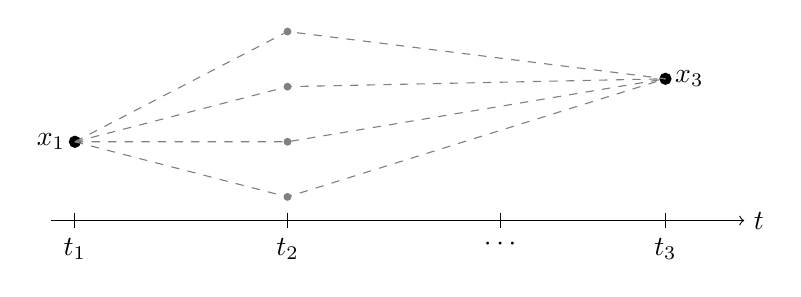
\begin{tikzpicture}[scale=1.0]
  % time axis
  \draw[->] (-0.3,0) -- (8.5,0) node[right]{$t$};
  \foreach \x/\lab in {0/{t_1}, 2.7/{t_2}, 5.4/{\cdots}, 7.5/{t_3}}{
     \draw (\x,0.1) -- (\x,-0.1) node[below]{$\lab$};
  }
  % start and end nodes
  \filldraw (0,1) circle (2pt) node[left]{$x_1$};
  \filldraw (7.5,1.8) circle (2pt) node[right]{$x_3$};
  % intermediate fan of possible values at t2
  \foreach \y in {0.3,1.0,1.7,2.4}{
     \draw[gray,dashed] (0,1) -- (2.7,\y) -- (7.5,1.8);
     \filldraw[gray] (2.7,\y) circle (1.2pt);
  }
\end{tikzpicture}
\caption{Chapman--Kolmogorov concatenation: every path from $(x_1,t_1)$ to $(x_3,t_3)$ is decomposed through all intermediate states at $t_2$, and one sums over them.}
\label{fig:chapman-kolmogorov}
\end{figure}

The Chapman--Kolmogorov equation is exact, but it is an integral equation for an unknown function of four arguments --- hardly something one solves directly.
The way forward is to expand it for infinitesimal time steps and turn it into a differential equation.
This is the Kramers--Moyal expansion, which we now derive.


\section{The Kramers--Moyal expansion}

We look for the equation according to which the density $P(x,t)$ evolves.
It is convenient to change notation in the Chapman--Kolmogorov equation~\eqref{eq:chapman-kolmogorov}: we rename
\begin{equation}
\begin{aligned}
x_1,t_1 &\longrightarrow x_0,t_0 && (x_0\ \text{fixed}),\\
x_2,t_2 &\longrightarrow x',t   && (x'\ \text{variable}),\\
x_3,t_3 &\longrightarrow x,t+\tau && (x\ \text{fixed}),\qquad \text{with } \tau \ll t-t_0,
\end{aligned}
\end{equation}
so that the roles are clear: the process started long ago at $x_0$, we watch it at time $t$, and we ask what happens a short instant $\tau$ later.
With this notation, subtracting $P(x,t\mid x_0,t_0)$ from both sides of Chapman--Kolmogorov gives
\begin{equation}
P(x,t+\tau\mid x_0,t_0) - P(x,t\mid x_0,t_0) = \int_{\mathbb{R}} dx'\, P(x,t+\tau\mid x',t)\,P(x',t\mid x_0,t_0) - P(x,t\mid x_0,t_0),
\end{equation}
and dividing by $\tau$ and letting $\tau\to0$ we recognize a time derivative on the left,
\begin{equation}\label{eq:km-limit}
\frac{\partial}{\partial t}P(x,t\mid x_0,t_0)
= \lim_{\tau\to0}\frac{1}{\tau}\left[\int_{\mathbb{R}} dx'\, P(x,t+\tau\mid x',t)\,P(x',t\mid x_0,t_0) - P(x,t\mid x_0,t_0)\right].
\end{equation}

Everything now hinges on the short-time transition density $P(x,t+\tau\mid x',t)$, which we expand.
Following Einstein's strategy from Chapter~2, define the increment $\Delta := x-x'$, so that $x=x'+\Delta$; the increment moves because $x'$ moves.
For the function
\begin{equation}
f(x') := P(x'+\Delta,t+\tau\mid x',t)\,P(x',t\mid x_0,t_0),
\end{equation}
the Taylor expansion around $x$ (with $x'-x=-\Delta$) reads
\begin{equation}
f(x') = \sum_{m=0}^{\infty} \frac{1}{m!}\,\frac{\partial^m f}{\partial x'^m}\bigg|_{x'=x}(x'-x)^m
       = \sum_{m=0}^{\infty} \frac{(-1)^m}{m!}\,\Delta^m\,\frac{\partial^m f}{\partial x^m}\bigg|_{x'=x}.
\end{equation}
Substituting into Equation~\eqref{eq:km-limit} and integrating over $\Delta$, we arrive at
\begin{equation}\begin{split}
&\frac{\partial}{\partial t}P(x,t\mid x_0,t_0)\\
&\quad= \lim_{\tau\to0}\frac{1}{\tau}\biggl\{\sum_{m=0}^{\infty}\frac{(-1)^m}{m!}\,\frac{\partial^m}{\partial x^m}\int_{\mathbb{R}} d\Delta\, \Delta^m\, P(x+\Delta,t+\tau\mid x,t)\,P(x,t\mid x_0,t_0)\\
&\qquad\quad - P(x,t\mid x_0,t_0)\biggr\}.
\end{split}\end{equation}
Let us examine the terms of the sum one by one.
The $m=0$ term is
\begin{equation}
\lim_{\tau\to0}\frac{1}{\tau}\left\{\int_{\mathbb{R}} d\Delta\, \underbrace{P(x+\Delta,t+\tau\mid x,t)}_{\text{normalized to } 1}\,P(x,t\mid x_0,t_0) - P(x,t\mid x_0,t_0)\right\} = 0,
\end{equation}
because the transition density is normalized, and the two terms cancel exactly.
The terms with $m\ge1$ survive the limit, and they define the \emph{Kramers--Moyal coefficients}
\begin{equation}
a_m(x,t) := \lim_{\tau\to0}\frac{1}{\tau}\int_{\mathbb{R}} d\Delta\, \Delta^m\, P(x+\Delta,t+\tau\mid x,t),
\end{equation}
which are nothing but the moments of the displacement per unit time.
Dimensional analysis already whispers their physical meaning: when $x$ is a position, $[a_1]=L\,T^{-1}$ and $[a_2]=L^2\,T^{-1}$, so $a_1$ has the dimensions of a \emph{velocity} and $a_2$ those of a \emph{diffusion} coefficient.
We will confirm this interpretation quantitatively in Section~\ref{sec:drift-diffusion}.
Typically the coefficients do not depend on time, in which case the process is called \emph{homogeneous}.

Putting everything together, we are left with the \emph{Kramers--Moyal expansion},
\begin{equation}
\frac{\partial}{\partial t}P(x,t\mid x_0,t_0) = \sum_{m=1}^{\infty} \frac{(-1)^m}{m!}\,\frac{\partial^m}{\partial x^m}\big[a_m(x,t)\,P(x,t\mid x_0,t_0)\big].
\label{eq:kramers-moyal}
\end{equation}
The Chapman--Kolmogorov integral equation has become a differential equation --- but of \emph{infinite} order.
The next section explains why, in practice, two terms are all we are allowed to keep.


\section{The Fokker--Planck equation}

Equation~\eqref{eq:kramers-moyal} is a differential (in fact integro-differential) equation of infinite order, hardly tractable; moreover any acceptable solution must satisfy $P(x,t\mid x_0,t_0)\ge0$, since it is a probability density.
One would like to simply truncate the series, but truncation is a delicate business: a theorem tells us exactly which truncations are legitimate.

\medskip
\noindent\textbf{Theorem (Pawula).}\cite{Pawula1967}
\emph{Only one of the following is admissible: the series truncated at first order, which gives the Liouville equation; the series truncated at second order, which gives the Fokker--Planck equation; or the full, untruncated series.}
\medskip

Any truncation at third order or beyond produces an ``evolution equation'' whose solutions become negative somewhere --- and a negative probability is no probability at all.
The theorem is therefore a great piece of luck: either the process is deterministic in disguise (Liouville), or the \emph{entire} statistics of its fluctuations is encoded in just two functions, $a_1$ and $a_2$.

Truncating at $m=1,2$ we obtain
\begin{equation}
\frac{\partial}{\partial t}P(x,t\mid x_0,t_0) = -\frac{\partial}{\partial x}\big[a_1(x,t)\,P(x,t\mid x_0,t_0)\big] + \frac{1}{2}\frac{\partial^2}{\partial x^2}\big[a_2(x,t)\,P(x,t\mid x_0,t_0)\big],
\label{eq:fokker-planck}
\end{equation}
which is the celebrated \emph{Fokker--Planck equation}, also known as the \emph{Kolmogorov forward equation} because it propagates the density forward in time, from $(x_0,t_0)$ towards the future.\cite{Risken1989,Gardiner2009}
This equation is the workhorse of the entire book.

Before moving on, one remark is in order.
By Bayes,
\begin{equation}
P(x_2,t_2\mid x_1,t_1)=\frac{P_2(x_2,t_2;x_1,t_1)}{P_1(x_1,t_1)},
\end{equation}
hence
\begin{equation}\begin{split}
\int_{\mathbb{R}} dx_1\, P_2(x_2,t_2;x_1,t_1) &= P_1(x_2,t_2)\\
&\overset{\text{compl.}}{=} \int_{\mathbb{R}} dx_1\, P(x_2,t_2\mid x_1,t_1)\,P_1(x_1,t_1),
\end{split}\end{equation}
from which one can derive the analogous expansion for the \emph{marginal} density,
\begin{equation}
\frac{\partial}{\partial t}P(x,t) = \sum_{m=1}^{\infty} \frac{(-1)^m}{m!}\,\frac{\partial^m}{\partial x^m}\big\{a_m(x,t)\,P(x,t)\big\}.
\end{equation}
This identity is \emph{always} true, for any stochastic process, because it uses nothing but Bayes.
The subtlety is what it is good for.
For a Markov process the transition probability determines everything, and the equation genuinely closes the dynamics.
For a non-Markov process the expansion still describes $P(x,t)$, but one would also need to know the entire past history to make predictions: the description is \emph{incomplete}.


\section{Probabilistic meaning of the Fokker--Planck equation}

A partial differential equation is only as good as our understanding of what it conserves.
Rewriting~\eqref{eq:fokker-planck} for the marginal density and collecting the spatial derivative,
\begin{equation}
\frac{\partial}{\partial t}P(x,t) + \frac{\partial}{\partial x}\underbrace{\left\{a_1(x,t)\,P(x,t) - \frac{1}{2}\frac{\partial}{\partial x}\big[a_2(x,t)\,P(x,t)\big]\right\}}_{\text{dimensions of a current}\ =:\ j(x,t)} = 0,
\end{equation}
we discover that the Fokker--Planck equation is a \emph{continuity equation},
\begin{equation}
\frac{\partial}{\partial t}P(x,t) + \frac{\partial}{\partial x}j(x,t) = 0,
\end{equation}
formally identical to the conservation laws of fluid dynamics or electromagnetism, with $j(x,t)$ playing the role of a \emph{probability current}.
To see what is being conserved, integrate over an interval $[a,b]$:
\begin{equation}
\frac{d}{dt}\int_a^b dx\, P(x,t) = -\int_a^b dx\, \frac{\partial}{\partial x}j(x,t) = j(a,t)-j(b,t),
\end{equation}
so probability can only change inside the interval by flowing through its endpoints.
It is physically reasonable to require $P(x,t)\xrightarrow{x\to\pm\infty}0$ with fast decay, and likewise $j(x,t)\to0$; therefore, letting $a\to-\infty$ and $b\to+\infty$,
\begin{equation}
\frac{d}{dt}\int_{\mathbb{R}} dx\, P(x,t) = 0,
\end{equation}
that is $\int_{\mathbb{R}} dx\, P(x,t) = \text{const}$, normalized to $1$.
The Fokker--Planck equation \emph{conserves probability}, just as the Schr\"odinger equation conserves the norm of the wave function.
For $t\to\infty$ the density may settle down, $P(x,t)\to P(x)$, and then $\partial_x j(x,t)=0$: this is the \emph{stationary} Fokker--Planck equation, whose equilibrium meaning --- detailed balance, and the Boltzmann form of the zero-flux state --- is developed in Appendix~\ref{app:stationary}, and which will be the key to the wealth distributions of Chapter~8.


\section{The drift and diffusion coefficients}
\label{sec:drift-diffusion}

We promised that $a_1$ acts as a velocity and $a_2$ as a diffusion coefficient; let us now prove it.
The tool is the pair of ensemble moments
\begin{equation}
\langle x(t)\rangle = \int_{\mathbb{R}} dx\, x\, P(x,t),\qquad
\langle x^2(t)\rangle = \int_{\mathbb{R}} dx\, x^2\, P(x,t),
\end{equation}
and for the moment we set $a_1(x,t)=:v$ and $a_2(x,t)=:D$, both constant.
Using the Fokker--Planck equation and integrating by parts (the boundary terms vanish thanks to the fast decay of $P$),
\begin{equation}\begin{split}
\frac{d}{dt}\langle x(t)\rangle &= \int_{\mathbb{R}} dx\, x\, \frac{\partial}{\partial t}P(x,t)\\
&\overset{\text{F--P}}{=} -v\int_{\mathbb{R}} dx\, x\, \frac{\partial}{\partial x}P(x,t) + \frac{D}{2}\int_{\mathbb{R}} dx\, x\, \frac{\partial^2}{\partial x^2}P(x,t) = v.
\end{split}\end{equation}
This is the analogue of the Ehrenfest theorem of quantum mechanics: the diffusion coefficient $D$ cannot contribute to the velocity of the mean, and
\begin{equation}
\frac{d}{dt}\langle x(t)\rangle = v \implies \langle x(t)\rangle = \langle x(0)\rangle + v\,t.
\end{equation}
The density keeps its shape and is simply transported at constant speed, as sketched in Figure~\ref{fig:drift}: this is why $v$ is called a \emph{drift} term.

\begin{figure}[h!]
\centering
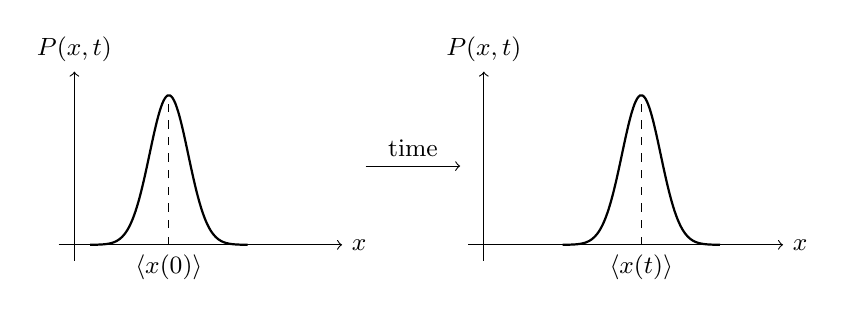
\begin{tikzpicture}[scale=1.0]
  \begin{scope}
    \draw[->] (-0.2,0) -- (3.4,0) node[right]{\small $x$};
    \draw[->] (0,-0.2) -- (0,2.2) node[above]{\small $P(x,t)$};
    \draw[thick,domain=0.2:2.2,smooth,samples=60] plot (\x,{1.9*exp(-(\x-1.2)^2/0.12)});
    \draw[dashed] (1.2,0) -- (1.2,1.9);
    \node[below] at (1.2,0) {\small $\langle x(0)\rangle$};
  \end{scope}
  \draw[->] (3.7,1) -- (4.9,1) node[midway,above]{\small time};
  \begin{scope}[xshift=5.2cm]
    \draw[->] (-0.2,0) -- (3.8,0) node[right]{\small $x$};
    \draw[->] (0,-0.2) -- (0,2.2) node[above]{\small $P(x,t)$};
    \draw[thick,domain=1.0:3.0,smooth,samples=60] plot (\x,{1.9*exp(-(\x-2.0)^2/0.12)});
    \draw[dashed] (2.0,0) -- (2.0,1.9);
    \node[below] at (2.0,0) {\small $\langle x(t)\rangle$};
  \end{scope}
\end{tikzpicture}
\caption{Pure drift: the density keeps the same shape and its mean is transported at constant velocity, $\langle x(t)\rangle=\langle x(0)\rangle+v\,t$.}
\label{fig:drift}
\end{figure}

The second moment tells the complementary story.
For pure diffusion ($v=0$), the same integration-by-parts routine gives
\begin{equation}\begin{split}
\frac{d}{dt}\langle x^2(t)\rangle &= \int_{\mathbb{R}} dx\, x^2\, \frac{\partial}{\partial t}P(x,t)
= \frac{D}{2}\int_{\mathbb{R}} dx\, x^2\, \frac{\partial^2}{\partial x^2}P(x,t)\\
&= -\frac{D}{2}\int_{\mathbb{R}} dx\, 2x\, \frac{\partial}{\partial x}P(x,t)
= D\int_{\mathbb{R}} dx\, P(x,t) = D,
\end{split}\end{equation}
so it makes sense to call $D$ a \emph{diffusion} coefficient, with
\begin{equation}
\langle x^2(t)\rangle = \langle x^2(0)\rangle + D\,t.
\end{equation}
The density now stays put but spreads, as in Figure~\ref{fig:diffusion}.

% Figure after the sketches in the handwritten notes (PDF 2), added 2026-07-06.
\begin{figure}[h!]
\centering
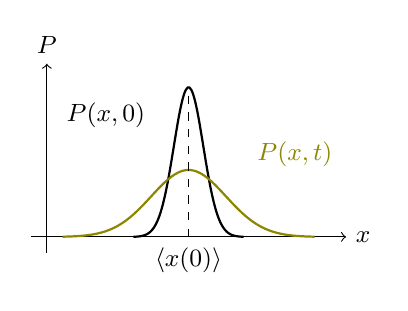
\begin{tikzpicture}[scale=1.0]
    \draw[->] (-0.2,0) -- (3.8,0) node[right]{\small $x$};
    \draw[->] (0,-0.2) -- (0,2.2) node[above]{\small $P$};
    \draw[thick,domain=1.1:2.5,smooth,samples=60] plot (\x,{1.9*exp(-(\x-1.8)^2/0.07)});
    \draw[thick,olive,domain=0.2:3.4,smooth,samples=60] plot (\x,{0.85*exp(-(\x-1.8)^2/0.45)});
    \draw[dashed] (1.8,0) -- (1.8,1.9);
    \node[below] at (1.8,-0.02) {\small $\langle x(0)\rangle$};
    \node[font=\small] at (0.75,1.55) {$P(x,0)$};
    \node[olive,font=\small] at (3.15,1.05) {$P(x,t)$};
\end{tikzpicture}
\caption{Pure diffusion ($v=0$): the density keeps its centre $\langle x(0)\rangle$ fixed and spreads, its variance growing linearly as $\langle x^2(t)\rangle = \langle x^2(0)\rangle + D\,t$.}
\label{fig:diffusion}
\end{figure}

If the motion is not purely diffusive there is also the drift contribution $\int dx\, x^2(-v\,\partial_x P) = 2v\langle x\rangle$, so that
\begin{equation}
\frac{d}{dt}\langle x^2(t)\rangle = D + 2v\langle x(t)\rangle = D + 2v\big(\langle x(0)\rangle + v\,t\big),
\end{equation}
and integrating in time,
\begin{equation}
\langle x^2(t)\rangle = \langle x^2(0)\rangle + D\,t + 2v\langle x(0)\rangle t + v^2 t^2.
\end{equation}
On the other hand $\langle x(t)\rangle^2 = \big[\langle x(0)\rangle + v\,t\big]^2 = \langle x(0)\rangle^2 + 2v\langle x(0)\rangle t + v^2 t^2$, and subtracting we find the clean statement
\begin{equation}
\mathrm{Var}[x(t)] = \langle x^2(t)\rangle - \langle x(t)\rangle^2 = \mathrm{Var}[x(0)] + D\,t.
\end{equation}
The drift drops out completely: the variance grows linearly in time, exactly as for diffusion, and only $D$ controls its rate.
Drift moves the crowd; diffusion spreads it.
In the general case both happen at once, as summarized in Figure~\ref{fig:drift-diffusion}: the density is transported at velocity $v$ \emph{and} broadens as it travels.

% Figure after the sketches in the handwritten notes (PDF 2), added 2026-07-06.
\begin{figure}[h!]
\centering
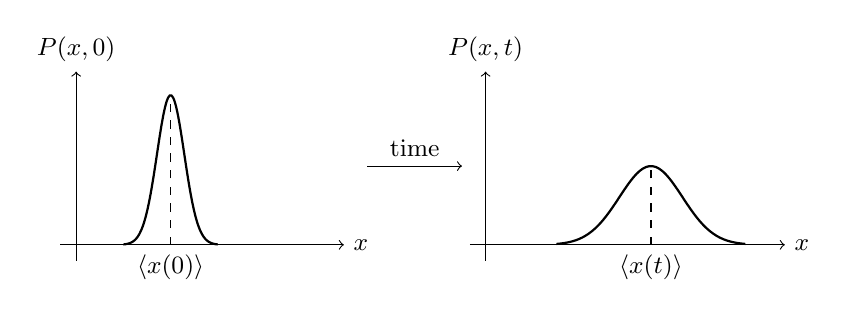
\begin{tikzpicture}[scale=1.0]
  \begin{scope}
    \draw[->] (-0.2,0) -- (3.4,0) node[right]{\small $x$};
    \draw[->] (0,-0.2) -- (0,2.2) node[above]{\small $P(x,0)$};
    \draw[thick,domain=0.6:1.8,smooth,samples=60] plot (\x,{1.9*exp(-(\x-1.2)^2/0.06)});
    \draw[dashed] (1.2,0) -- (1.2,1.9);
    \node[below] at (1.2,0) {\small $\langle x(0)\rangle$};
  \end{scope}
  \draw[->] (3.7,1) -- (4.9,1) node[midway,above]{\small time};
  \begin{scope}[xshift=5.2cm]
    \draw[->] (-0.2,0) -- (3.8,0) node[right]{\small $x$};
    \draw[->] (0,-0.2) -- (0,2.2) node[above]{\small $P(x,t)$};
    \draw[thick,domain=0.9:3.3,smooth,samples=60] plot (\x,{1.0*exp(-(\x-2.1)^2/0.32)});
    \draw[dashed] (2.1,0) -- (2.1,1.0);
    \node[below] at (2.1,0) {\small $\langle x(t)\rangle$};
  \end{scope}
\end{tikzpicture}
\caption{The general case, drift and diffusion together: the density is transported ($\langle x(t)\rangle = \langle x(0)\rangle + v\,t$) while it spreads ($\mathrm{Var}[x(t)] = \mathrm{Var}[x(0)] + D\,t$).}
\label{fig:drift-diffusion}
\end{figure}

For coefficients that genuinely depend on $x$ and $t$, the same computation yields the general laws
\begin{equation}
\frac{d}{dt}\langle x(t)\rangle = \langle a_1(x,t)\rangle,\qquad
\frac{d}{dt}\langle x^2(t)\rangle = 2\langle x\,a_1(x,t)\rangle + \langle a_2(x,t)\rangle.
\end{equation}
How easy the Fokker--Planck equation is to solve depends entirely on the functional forms of $a_1(x,t)$ and $a_2(x,t)$; a small catalogue of the important cases is given in Section~\ref{sec:general-solution-fp}.


\section{The Wiener process}

The simplest non-trivial choice of coefficients is
\begin{equation}
a_1(x,t)=0,\qquad a_2(x,t)=1,
\end{equation}
that is, pure diffusion with unit diffusion coefficient: this defines the \emph{Wiener process}.
The Fokker--Planck equation to solve is
\begin{equation}
\frac{\partial}{\partial t}P(x,t\mid x_0,t_0) = \frac{1}{2}\frac{\partial^2}{\partial x^2}P(x,t\mid x_0,t_0),
\qquad P(x,t_0\mid x_0,t_0)=\delta(x-x_0),
\end{equation}
which is exactly the heat-equation problem already solved in Chapter~2, with solution
\begin{equation}
P(x,t\mid x_0,t_0) = \frac{1}{\sqrt{2\pi(t-t_0)}}\,e^{-\frac{(x-x_0)^2}{2(t-t_0)}}.
\end{equation}
The process is often also called Brownian motion, although --- as we shall see at the end of this section --- somewhat improperly.

It is convenient to change the point of view from positions to \emph{increments}.
Introducing
\begin{equation}
\Delta t_i := t_i - t_{i-1},\qquad \Delta x_i := x_i - x_{i-1},
\end{equation}
the transition density reads
\begin{equation}\begin{split}
P(x_i,t_i\mid x_{i-1},t_{i-1}) &= \frac{1}{\sqrt{2\pi(t_i-t_{i-1})}}\,e^{-\frac{(x_i-x_{i-1})^2}{2(t_i-t_{i-1})}}\\
&= \frac{1}{\sqrt{2\pi\,\Delta t_i}}\,e^{-\frac{\Delta x_i^2}{2\Delta t_i}}
= P(\Delta x_i,\Delta t_i) = \mathcal{N}(0,\Delta t_i),
\end{split}\end{equation}
so the \emph{conditional} density of the positions has become the \emph{marginal} density of the increments: each increment is a Gaussian of zero mean and variance equal to the elapsed time, regardless of where the process currently sits.
This innocent-looking rewriting is the source of all the properties that follow.

\paragraph{a) Stationary increments.}
Sending $t_{i-1}\to t_{i-1}+\Delta t$ and $t_i\to t_i+\Delta t$ leaves the density unchanged: the increments are invariant under time translation.
Note that the process itself is \emph{not} stationary in the strong sense --- its variance grows without bound --- but its increments are.

\paragraph{b) Independent increments.}
By the Markov property,
\begin{equation}\begin{split}
P_n(x_n,t_n;\dots;x_0,t_0) &= \prod_{i=1}^{n} P(x_i,t_i\mid x_{i-1},t_{i-1})\,P(x_0,t_0)\\
&= \prod_{i=1}^{n} \frac{1}{\sqrt{2\pi\,\Delta t_i}}\,e^{-\frac{\Delta x_i^2}{2\Delta t_i}}\,P(x_0,t_0)\\
&= \prod_{i=1}^{n} P(\Delta x_i,\Delta t_i)\,P(x_0,t_0),
\end{split}\end{equation}
which is a product of $n$ densities of identical functional form.
Given $x_0$, one reconstructs $x_1 = x_0+\Delta x_1$, $x_2 = x_1+\Delta x_2,\ \dots,\ x_i = x_{i-1}+\Delta x_i$; once $x_0$ is fixed, all the positions can be recovered from the increments, so that
\begin{equation}
P_n(x_n,t_n;\dots;x_0,t_0) = P_n(\Delta x_n,\Delta t_n;\dots;x_0,t_0),
\end{equation}
but the factorized form holds \emph{only because} the increments are independent.
If, moreover, the spacing is uniform, $\Delta t := (t_m-t_0)/m$, then $P(\Delta x_i,\Delta t)=\mathcal{N}(0,\Delta t)$ for every $i$, and the increments become independent \emph{and} identically distributed --- the i.i.d.\ setting in which all of elementary probability applies.

\paragraph{c) Scale invariance.}
Start again from
\begin{equation}
P(x,t\mid x_0,t_0) = \frac{1}{\sqrt{2\pi(t-t_0)}}\,e^{-\frac{(x-x_0)^2}{2(t-t_0)}},
\end{equation}
let $b\in\mathbb{R}^+$ be a scaling factor, and stretch time and space in the coordinated way
\begin{equation}
t-t_0 \to b(t-t_0) = \hat t - \hat t_0,\qquad x-x_0 \to \sqrt{b}\,(x-x_0) = \hat x - \hat x_0.
\end{equation}
Then
\begin{equation}\begin{split}
\hat P(\hat x,\hat t\mid \hat x_0,\hat t_0) &= \frac{1}{\sqrt{2\pi\,b(t-t_0)}}\,e^{-\frac{b(x-x_0)^2}{2b(t-t_0)}}\\
&= b^{-1/2}\,\frac{1}{\sqrt{2\pi(t-t_0)}}\,e^{-\frac{(x-x_0)^2}{2(t-t_0)}} = b^{-1/2}\,P(x,t\mid x_0,t_0),
\end{split}\end{equation}
and checking the normalization,
\begin{equation}
\int d\hat x\, \hat P(\hat x,\hat t\mid \hat x_0,\hat t_0) = \int dx\, b^{1/2}\,b^{-1/2}\,P(x,t\mid x_0,t_0) = 1,
\end{equation}
so the rescaled density is still a normalized density with the same moments.
Zooming into a Wiener trajectory with the right anisotropic magnification ($\sqrt{b}$ in space for every factor $b$ in time) reproduces a statistically identical trajectory: the Wiener process is \emph{self-similar}, a one-dimensional fractal process.
This is why plots of stock prices look qualitatively the same at the scale of a day or of a year.

\paragraph{d) Continuity of the trajectories.}
We now ask whether an individual trajectory is continuous.
Let $t=t_{i-1}$, $x(t)=x_{i-1}$, $\Delta t=t_i-t_{i-1}$, $\Delta x=x_i-x_{i-1}$, so that $t_i=t+\Delta t$ and $x_i=x+\Delta x$.
The trajectory $X(t)$ is discontinuous if and only if there exists $k>0$ such that $|x(t+\Delta t)-x(t)|>k$ as $\Delta t\to0$ with nonzero probability --- in words, if finite jumps survive the limit of vanishing time step.
Writing the increment $W:=\Delta x$, the probability of such a jump is
\begin{equation}
\mathrm{Prob}\{|W|>k\} = \int_{|W|>k} dW\, \frac{1}{\sqrt{2\pi\,\Delta t}}\,e^{-\frac{|W|^2}{2\Delta t}},
\end{equation}
over the symmetric integration domain $(-\infty,-k)\cup(k,+\infty)$, hence
\begin{equation}
\mathrm{Prob}\{|W|>k\} = \frac{2}{\sqrt{2\pi\,\Delta t}}\int_k^{+\infty} dW\, e^{-\frac{W^2}{2\Delta t}}.
\end{equation}
Recalling the error function and its complement,
\begin{equation}
\mathrm{erf}(x) = \frac{2}{\sqrt{\pi}}\int_0^x dt\, e^{-t^2},\qquad
\mathrm{erfc}(x) = 1-\mathrm{erf}(x) = \frac{2}{\sqrt{\pi}}\int_x^{\infty} dt\, e^{-t^2},
\end{equation}
and substituting $W\to W' = W/\sqrt{2\Delta t}$, $dW=\sqrt{2\Delta t}\,dW'$, we obtain
\begin{equation}
\mathrm{Prob}\{|W|>k\} = \frac{2\sqrt{2\Delta t}}{\sqrt{2\pi\cdot 2\Delta t}}\int_{k/\sqrt{2\Delta t}}^{+\infty} dW'\, e^{-W'^2}
= \mathrm{erfc}\!\left(\frac{k}{\sqrt{2\Delta t}}\right) \xrightarrow{\ \Delta t\to0\ } 0.
\end{equation}
The trajectories are discontinuous with probability $0$, i.e.\ \emph{continuous with probability $1$} (almost surely).

\paragraph{e) Differentiability of the trajectories.}
Continuity secured, the natural next question is whether the trajectories have a velocity.
Consider
\begin{equation}
\lim_{\Delta t\to0}\frac{x(t+\Delta t)-x(t)}{\Delta t} = \lim_{\Delta t\to0}\frac{|W|}{\Delta t};
\end{equation}
the trajectory $X(t)$ is non-differentiable if and only if $\lim_{\Delta t\to0}\mathrm{Prob}\{|W|/\Delta t>k\}$ stays finite for every $k>0$.
The same computation as in (d), with $k$ replaced by $k\,\Delta t$, gives
\begin{equation}\begin{split}
\mathrm{Prob}\left\{\frac{|W|}{\Delta t}>k\right\} &= \frac{1}{\sqrt{2\pi\,\Delta t}}\int_{k\Delta t}^{+\infty} dW\, e^{-\frac{W^2}{2\Delta t}}\\
&= \mathrm{erfc}\!\left(\frac{k\Delta t}{\sqrt{2\Delta t}}\right) = \mathrm{erfc}\!\left(k\sqrt{\tfrac{\Delta t}{2}}\right) \xrightarrow{\ \Delta t\to0\ } 1,
\qquad \forall k\in\mathbb{R}^+.
\end{split}\end{equation}
The probability that the difference quotient exceeds \emph{any} threshold tends to one: the limit never exists, and the trajectories are almost surely \emph{non-differentiable}.

This last property deserves a pause.
If the Wiener process were the physical trajectory of Einstein's Brownian particle, the particle would have $dx/dt = v \to \infty$ at every instant --- an infinite instantaneous velocity.
The Wiener process is therefore an admirable mathematical idealization, but it \emph{cannot} be the literal physical representation of Brownian motion; and its non-differentiability is precisely what will force us, in the next chapter, to invent a new calculus.


\section{A rigorous definition of the Wiener process}

So far the Wiener process has been defined through its Fokker--Planck equation.
Modern probability theory prefers an axiomatic characterization, which we record here because it is the form used in the mathematical finance literature.
From a purely stochastic point of view, the \emph{Wiener process} $W(t)$ (also denoted $B(t)$) is a continuous-time stochastic process $\{W(t)\}_{t\ge0}$ such that:
\begin{enumerate}[label=(\roman*)]
    \item $W(0)=0$ almost surely;
    \item the trajectories are continuous almost surely;
    \item the process has \emph{independent increments}: for $s'\le t'\le s\le t$, the increments $W(t)-W(s)$ and $W(t')-W(s')$ are independent;
    % CLAUDE NOTE: the notes write the index ordering in a condensed and partly ambiguous way;
    % the standard statement (independence of increments over disjoint time intervals) is used here.
    \item $W(t)-W(s)\sim\mathcal{N}(0,\,t-s)$ for $t>s$.
\end{enumerate}
One checks easily that these axioms reproduce everything derived in the previous section.

The increments are independent; but are the \emph{positions} independent as well?
Intuition says no --- where the process can be now depends on where it was --- and the autocorrelation function confirms it.
Writing $W(t)=W(s)+[W(t)-W(s)]$ and using $W(s)=W(s)-W(0)$,
\begin{equation}\begin{split}
\langle W(t)W(s)\rangle &= \big\langle\,[W(t)-W(s)]\,W(s)\,\big\rangle + \langle W^2(s)\rangle\\
&= \underbrace{\big\langle\,[W(t)-W(s)]\,[W(s)-W(0)]\,\big\rangle}_{\text{independent increments}} + \langle W^2(s)\rangle.
\end{split}\end{equation}
The two increments $W(t)-W(s)$ and $W(s)-W(0)$ live on disjoint time intervals, so they are independent and both have zero mean; the first term vanishes and only the second moment survives.
Now, with $\Delta W(s)=W(s)-W(0)$ and $\langle\Delta W(s)\rangle=0$,
\begin{equation}\begin{split}
\mathrm{Var}[\Delta W(s)] &= \big\langle\big(\Delta W(s)-\langle\Delta W(s)\rangle\big)^2\big\rangle\\
&= \big\langle\big(W(s)-W(0)\big)^2\big\rangle = \langle W^2(s)\rangle,
\qquad \mathrm{Var}[W(s)] = s,
\end{split}\end{equation}
hence $\langle W(t)W(s)\rangle = s$ --- but only for $s<t$; exchanging the roles of $s$ and $t$ gives the symmetric result, and in general
\begin{equation}\begin{split}
\langle W(t)W(s)\rangle &= \min(t,s),\\
\mathrm{Cov}[W(t),W(s)] &= \langle W(t)W(s)\rangle - \langle W(s)\rangle\langle W(t)\rangle = \min(t,s).
\end{split}\end{equation}
The corresponding correlation coefficient is
\begin{equation}
\rho = \frac{\mathrm{Cov}[W(t),W(s)]}{\sigma_{W(t)}\,\sigma_{W(s)}} = \frac{\min(s,t)}{\sqrt{s\,t}} \xrightarrow{\ t,s\to\infty\ } 0.
\end{equation}
The positions are therefore \emph{not} independent: they are the more correlated the closer the two times are, and the memory fades --- but only slowly --- as the times drift apart.
The curious formula $\langle W(t)W(s)\rangle=\min(t,s)$ will return in the next chapter, where its distributional derivatives generate the white noise.


\section{General solution of the Fokker--Planck equation}
\label{sec:general-solution-fp}

How the Fokker--Planck equation~\eqref{eq:fokker-planck} is solved depends on the functional forms of the coefficients $a_1(x,t)$ and $a_2(x,t)$, and it is worth having a small catalogue of the cases that will matter to us.
\begin{enumerate}
    \item $a_1=0$, $a_2\in\{1,D\}$: pure diffusion, i.e.\ the heat equation, which we have already solved.
    \item $a_1=v$, $a_2\in\{1,D\}$: constant drift plus diffusion, solved by Fourier transform.
    \item $a_1(x,t)=-\gamma x$, $a_2=D$ with $\gamma>0$: a linear restoring drift; this is the \emph{Ornstein--Uhlenbeck process},\cite{UhlenbeckOrnstein1930} harder to solve but feasible, and ubiquitous in what follows.
    \item $a_1(x)=\kappa(\theta-x)$, $a_2(x)=\sigma^2 x$: the \emph{CIR process},\cite{CIR1985} with a linear mean-reverting drift and a diffusion that switches off as $x\to0$.
    % CLAUDE NOTE: the notes write a_1 = -gamma*sqrt(x), a_2 = D; corrected at the author's
    % request (2026-07-06) to the standard CIR form, which is also the one consistently
    % derived in Chapter 6 via Itô from an OU process for sqrt(r).
    \item $a_1(x,t)=ax$, $a_2(x,t)=\sigma^2 x^2$: the \emph{geometric Brownian motion} (GBM), whose solution is not Gaussian; it will be the standard model for stock prices from Chapter~5 onwards.
\end{enumerate}

Case-by-case tricks are all well and good, but one would like a \emph{general} strategy, valid for arbitrary coefficients.
There is one, and it proceeds in two steps: first we find the transition probability over an infinitesimally short time, where everything can be computed explicitly; then we chain infinitely many short steps together with Chapman--Kolmogorov, which produces a \emph{path integral} in the style of Wiener and Kac.
We take the two steps in turn.

\subsection{Short-time transition probability}

It is convenient to write the Fokker--Planck equation in operator form,
\begin{equation}
\frac{\partial}{\partial t}P(x,t\mid x',t_0) = L_{\mathrm{FP}}(x,t)\,P(x,t\mid x',t_0),\qquad
L_{\mathrm{FP}}(x,t) = -\frac{\partial}{\partial x}a_1(x,t) + \frac{1}{2}\frac{\partial^2}{\partial x^2}a_2(x,t),
\end{equation}
where $L_{\mathrm{FP}}$ is called the Fokker--Planck operator.
Integrating formally in time,
\begin{equation}
P(x,t\mid x',t_0) = P(x,t_0\mid x',t_0) + \int_{t_0}^{t} dt'\, L_{\mathrm{FP}}(x,t')\,P(x,t'\mid x',t_0),
\end{equation}
which is an integral equation whose unknown appears on both sides --- an invitation to iterate.
Taking the initial condition $P(x,t_0\mid x',t_0):=\delta(x-x')$ and substituting the equation into itself repeatedly,
\begin{equation}
\begin{aligned}
P(x,t\mid x',t_0) =\ & \delta(x-x') + \int_{t_0}^{t} dt'\, L_{\mathrm{FP}}(x,t')\,\delta(x-x')\\
& + \int_{t_0}^{t} dt'\int_{t_0}^{t'} dt''\, L_{\mathrm{FP}}(x,t')\,L_{\mathrm{FP}}(x,t'')\,\delta(x-x') + \dots,
\end{aligned}
\end{equation}
which the reader may recognize as a \emph{Dyson expansion}, the same structure that appears in time-dependent perturbation theory in quantum mechanics.
If $L_{\mathrm{FP}}$ does not depend on time, $a_i(x,t)=a_i(x)$, the series resums neatly into an exponential,
\begin{equation}
P(x,t\mid x',t_0) = \exp\!\big[L_{\mathrm{FP}}(x)\,(t-t_0)\big]\,\delta(x-x'),
\end{equation}
while at first order
\begin{equation}
P(x,t\mid x',t_0) \approx \delta(x-x') + \int_{t_0}^{t} dt'\, L_{\mathrm{FP}}(x,t')\,\delta(x-x').
\end{equation}
Setting $\tau := t-t_0$, each term of the series carries a factor $t-t_0$: if the interval $[t_0,t]$ is very small, the area under $L_{\mathrm{FP}}(x,t')$ is approximately a rectangle,
\begin{equation}
\int_{t_0}^{t} dt'\, L_{\mathrm{FP}}(x,t') \approx \tau\,L_{\mathrm{FP}}(x,t) + \text{higher-order infinitesimals},
\end{equation}
and the truncation at first order becomes accurate.
Then for a generic short transition $t\to t+\tau$,
\begin{equation}
P(x,t+\tau\mid x',t) \approx \delta(x-x') + L_{\mathrm{FP}}(x,t)\,\tau\,\delta(x-x') = \big\{1 + L_{\mathrm{FP}}(x,t)\,\tau\big\}\delta(x-x'),
\end{equation}
or, writing the operator out explicitly,
\begin{equation}
P(x,t+\tau\mid x',t) \approx \delta(x-x') - \frac{\partial}{\partial x}\big\{a_1(x,t)\,\delta(x-x')\big\}\tau + \frac{1}{2}\frac{\partial^2}{\partial x^2}\big\{a_2(x,t)\,\delta(x-x')\big\}\tau.
\end{equation}

This is a formula built out of derivatives of delta functions --- can one pass from this distributional form to an honest analytic one?
Yes, and legitimately so, because the expression only ever appears under an integral.
For any test function $f(x)$ the delta acts as $f(x)\delta(x-x')=f(x')\delta(x-x')$; applying this with $f(x)=a_i(x,t)$ frees the coefficients from the derivatives,
\begin{equation}
P(x,t+\tau\mid x',t) \approx \left\{1 - \frac{\partial}{\partial x}a_1(x',t)\,\tau + \frac{1}{2}\frac{\partial^2}{\partial x^2}a_2(x',t)\,\tau\right\}\delta(x-x').
\end{equation}
Now we use the Fourier representation $\delta(x-x')=\frac{1}{2\pi}\int_{\mathbb{R}} dk\, e^{ik(x-x')}$, under which each $\partial_x$ becomes a factor $ik$, and then re-exponentiate ($e^{z}=1+z+\dots$, accurate to the same order in $\tau$):
\begin{equation}
\begin{aligned}
P(x,t+\tau\mid x',t)
&\approx \frac{1}{2\pi}\int_{\mathbb{R}} dk\, \left\{1 - i k\,a_1(x',t)\,\tau - \tfrac{1}{2}k^2\,a_2(x',t)\,\tau\right\} e^{ik(x-x')}\\
&\approx \frac{1}{2\pi}\int_{\mathbb{R}} dk\, e^{\,ik\big(x-x'-a_1(x',t)\tau\big) - \frac{1}{2}k^2 a_2(x',t)\tau}\\
&= \frac{1}{\sqrt{2\pi\,a_2(x',t)\,\tau}}\,\exp\!\left\{-\frac{\big[x-x'-a_1(x',t)\,\tau\big]^2}{2\,a_2(x',t)\,\tau}\right\},
\end{aligned}
\end{equation}
where the last step is the standard Gaussian integral in $k$.
The result is beautifully transparent: over a short time $\tau$, \emph{any} diffusion process looks Gaussian, with mean $x'+a_1(x',t)\,\tau$ (the particle drifts) and variance $a_2(x',t)\,\tau$ (the particle diffuses).
Without drift ($a_1=0$) one recovers exactly the Einstein--Wiener solution.
All the complications of a general Fokker--Planck equation come from chaining these elementary Gaussian steps together --- which is precisely what we do next.

\subsection{Path integral and the Wiener measure}

Can the short-time result be applied to a generic, not necessarily small, interval $[t_0,t]$?
Not directly; but Chapman--Kolmogorov tells us how to compose short steps into long ones.
Introducing an intermediate time $t_1$,
\begin{equation}
P(x,t\mid x_0,t_0) = \int_{\mathbb{R}} dx_1\, P(x,t\mid x_1,t_1)\,P(x_1,t_1\mid x_0,t_0),
\end{equation}
and iterating with a second intermediate time $t_2$,
\begin{equation}
P(x,t\mid x_0,t_0) = \int_{\mathbb{R}} dx_1\int_{\mathbb{R}} dx_2\, P(x,t\mid x_2,t_2)\,P(x_2,t_2\mid x_1,t_1)\,P(x_1,t_1\mid x_0,t_0),
\end{equation}
with three sub-intervals and three conditional densities.
Continuing with uniform spacing $\Delta t=(t-t_0)/N$, so that $t_0+N\Delta t = t = t_N$ and $t_0<t_1<\dots<t_N=t$,
\begin{equation}
P(x,t\mid x_0,t_0) = \int_{\mathbb{R}} dx_1\cdots\int_{\mathbb{R}} dx_{N-1}\, \prod_{k=1}^{N} P(x_k,t_k\mid x_{k-1},t_{k-1}),
\end{equation}
which we write compactly as a \emph{functional integral} over all trajectories,
\begin{equation}
P(x,t\mid x_0,t_0) = \int \mathcal{D}_\alpha x\, \prod_{k=1}^{N} P(x_k,t_k\mid x_{k-1},t_{k-1}).
\end{equation}
The formal limit
\begin{equation}
N\to\infty,\qquad \Delta t\to0,\qquad N\Delta t = t-t_0\ \text{finite},
\end{equation}
defines the \emph{Wiener measure} on the space of trajectories.
Each factor in the product is now a \emph{short-time} propagator, for which we may insert the Gaussian found above (valid for $\Delta t\ll t-t_0$),
\begin{equation}
P(x_k,t_k\mid x_{k-1},t_{k-1}) \approx \frac{1}{\sqrt{2\pi\,a_2(x_{k-1},t_{k-1})\,\Delta t}}\,\exp\!\left\{-\frac{\big[x_k-x_{k-1}-a_1(x_{k-1},t_{k-1})\Delta t\big]^2}{2\,a_2(x_{k-1},t_{k-1})\,\Delta t}\right\},
\end{equation}
and using $\prod_k e^{S_k}=e^{\sum_k S_k}$ the product of exponentials becomes the exponential of a sum,
\begin{equation}
P(x,t\mid x_0,t_0) = \lim_{N\to\infty}\int \mathcal{D}_\alpha x\, \prod_{k=1}^{N}\frac{1}{\sqrt{2\pi\,a_2(x_{k-1},t_{k-1})\,\Delta t}}\,\exp\!\left\{\sum_{k=1}^{N} S_k\right\},
\end{equation}
with
\begin{equation}
S := \sum_{k=1}^{N} S_k = -\sum_{k=1}^{N}\frac{1}{2\,a_2(x_{k-1},t_{k-1})}\left[\frac{x_k-x_{k-1}}{\Delta t}-a_1(x_{k-1},t_{k-1})\right]^2\Delta t.
\end{equation}
Thus $P(x,t\mid x_0,t_0)\sim e^{S}$, and $S$ plays the role of an \emph{action}: each term has the structure
\begin{equation}
-\frac{\big[x_k-x_{k-1}-a_1\,\Delta t\big]^2}{2\,a_2\,\Delta t} = -\frac{1}{2\,a_2}\left[\frac{\Delta x}{\Delta t}-a_1\right]^2\Delta t,
\end{equation}
a squared ``velocity mismatch'' weighted by the inverse diffusion.
In the continuum limit $\sum_{k=1}^{N}(\cdots)\Delta t \to \int_{t_0}^{t} dt'$ and $\Delta x/\Delta t \to \dot x(t)$, hence
\begin{equation}
S[x(t)] = \int_{t_0}^{t} dt'\, \left\{-\frac{1}{2\,a_2(x,t)}\big(\dot x - a_1(x,t)\big)^2\right\},
\end{equation}
and finally
\begin{equation}
P(x,t\mid x_0,t_0) = \int \mathcal{D}[x(t)]\, \exp\!\left\{-\int_{t_0}^{t} \mathcal{L}_{\mathrm{OM}}(x,\dot x,t)\,dt'\right\},
\end{equation}
where
\begin{equation}
\mathcal{L}_{\mathrm{OM}} = \frac{\big(\dot x - a_1(x,t)\big)^2}{2\,a_2(x,t)}
\end{equation}
is the \emph{Onsager--Machlup Lagrangian}.\cite{OnsagerMachlup1953}
The interpretation is worth savouring: every conceivable trajectory from $(x_0,t_0)$ to $(x,t)$ contributes, but trajectories whose velocity strays far from the local drift $a_1$ are exponentially suppressed, the more severely the smaller the diffusion $a_2$.
With $a_1=0$ and $a_2=1/m$ one gets $\mathcal{L}=\tfrac{1}{2}m\dot x^2$, formally the Lagrangian of a free particle in classical mechanics.

\subsection{Properties and equivalence}

The formula just found always holds; it is called the \emph{Wiener integral solution} of the Fokker--Planck equation, and three of its features deserve emphasis.
First, it is automatically normalized and positive definite: the exponential is positive, and the construction preserves normalization at every step --- so the constraint $P\ge0$, which made truncating Kramers--Moyal so delicate, here comes for free.
Second, it is a genuine functional integral, formally defined with the Wiener measure $\mathcal{D}x(t)$.
Third, and most importantly, it closes a conceptual loop: starting from Chapman--Kolmogorov there are \emph{two equivalent routes} to the dynamics --- the Kramers--Moyal expansion, which leads to the Fokker--Planck \emph{differential} equation, and the short-time transition probability, which leads to the path-integral, i.e.\ \emph{integral}, representation.
One must also be able to travel back and recover the Fokker--Planck equation from the path integral; this can indeed be shown, using the fact that the contributing trajectories are continuous and non-differentiable.

We close with a remark for the reader coming from quantum mechanics.
There is a profound difference between the Wiener--Kac construction, whose weight $e^{S}$ is \emph{real} and hence directly a probability density, and the Feynman construction, whose weight $e^{iS}$ is a complex \emph{amplitude} (which becomes classical only in the limit $\hbar\to0$).
Here the weight is $e^{S}$, and by integrating over all trajectories one can reconstruct any distribution of interest.
With this machinery --- Fokker--Planck on one side, trajectories on the other --- we are ready to ask the question that opens the next chapter: what is the differential equation obeyed by a \emph{single} trajectory?
